\documentclass{beamer}
% \linespread{1.3}

\mode<presentation>{
\usetheme{Madrid}
\usecolortheme{default}
%\usecolortheme{beaver}
}
\usepackage[utf8]{inputenc}
\usepackage{utopia}
\usepackage{verbatim}
\usepackage[portuguese]{babel}
\usepackage{pgfplots}
\pgfplotsset{/pgf/number format/use comma,compat=newest}
\usepackage{color}
\usepackage{amsmath,amsfonts,amssymb}
\usepackage{hyperref}
\usepackage{tikz}
\usepackage{caption}
\usepackage{soul}
%https://www.overleaf.com/project/61717826e515873b24296576
\usepackage{graphicx}
\usepackage{algorithm2e}
\usepackage{algorithmic}
\usetikzlibrary{positioning}

\setlength{\parskip}{1em}

\newcommand\ldiaarg[1]{\langle#1\rangle}

\newcommand{\M}{\mathcal{M}}
\newcommand{\LL}{\mathcal{L}} %for automata

\newcommand{\POL}{\mathsf{POL}}
\newcommand{\Decide}{\mathsf{Decide}}
\newcommand{\DecidePSPACE}{\mathsf{mcPOL}}
\newcommand{\reach}{\mathsf{PSPACEReach}}
\newcommand{\CreateDelta}{\mathsf{CreateDelta}}
\newcommand{\StringRepresent}{\mathsf{StringRepresent}}
\newcommand{\StoreStrings}{\mathsf{StoreStrings}}
\newcommand{\ResidueByLetter}{\mathsf{ResidueByLetter}}
\newcommand{\ResidueByWord}{\mathsf{ResidueByWord}}
\newcommand{\AuxOut}{\mathsf{AuxOut}}
\newcommand{\GetSetNP}{\mathsf{GetSetNP}}
\newcommand{\T}{\mathsf{True}}
\newcommand{\Fa}{\mathsf{False}}
\newcommand{\tr}{\mathsf{tr}}
\newcommand{\starfree}{\mathsf{Star\mbox{-}Free}}
\newcommand{\word}{\mathsf{Word}}
\newcommand{\existential}{\mathsf{Existential}}
\newcommand{\PSPACE}{\mathsf{PSPACE}}
\newcommand{\NPSPACE}{\mathsf{NPSPACE}}
\newcommand{\PTime}{\mathsf{P}}
\newcommand{\NP}{\mathsf{NP}}
\newcommand{\PTIME}{\mathsf{PTIME}}
\newcommand{\automaton}{\mathcal A}
\newcommand{\modelM}{\mathcal M}
\newcommand{\languageof}[1]{L({#1})}
\newcommand{\set}[1]{\{#1\}}
\newcommand{\suchthat}{\mid}
\newcommand{\union}{\cup}
\newcommand{\Union}{\bigcup}
\newcommand{\ep}{\ensuremath{\varepsilon}}

\newcommand{\obsright}{\blacktriangleright}
\newcommand{\obsleft}{\blacktriangleleft}
\newcommand{\obsup}{\blacktriangle}
\newcommand{\obsdown}{\blacktriangledown}

\newcommand{\expwater}{(\obsright \union \obsup)^* (\obsdown \union \obsleft \union \ep) (\obsright \union \obsup)^*}
\newcommand{\exppower}{(\obsleft \union \obsdown)^* (\obsup \union \obsright \union \ep) (\obsleft \union \obsdown)^*}
\newcommand{\exppatrol}{(\obsright^+ \obsdown^+ \obsleft^+ \obsup^+)^*}

\newcommand\algoaccept{\textbf{accept}}
\newcommand\algoreject{\textbf{reject}}

\tikzstyle{rectNode} = [rectangle, text centered]
\tikzstyle{fastate} = [circle, text centered, draw = black]
\tikzstyle{dots} = [circle, draw = black, fill = black, inner sep=1pt]

\tikzstyle{world} = [draw]

\makeatletter
\let\HL\hl
\renewcommand\hl{%
  \let\set@color\beamerorig@set@color
  \let\reset@color\beamerorig@reset@color
  \HL}
\makeatother



\title[On verifying expectations and observations of intelligent agents]{On verifying expectations and observations of intelligent agents}
\author[Avijeet Ghosh]{Avijeet Ghosh\\Joint work with Sourav Chakraborty, Sujata Ghosh and François Schwarzentruber}
\institute[ISI, Kolkata]{Indian Statistical Institute, Kolkata}
\date{}

\begin{document}

\begin{frame}
 \maketitle
\end{frame}

% \begin{frame}
% \frametitle{Table of Contents}
%  \tableofcontents
% \end{frame}

% \section{Introduction}

% \begin{frame}{Introduction: Logic}
%     \begin{itemize}
%         \item<1-> Formally modelling a real-world scenario, along with some rules that they follow, and some basic facts that are \textbf{valid} in it.
        
%         \item<2-> Able to reason, within the bounds of this scenario, using the rules and facts, to deduct new facts about the scenario.
        
%         \item<3-> Given a \textbf{property}, verify whether it is true in the system.
        
%         \item<5-> What property about the scenario can be \textbf{expressed} using the current system?
        
%         \item<6-> Does there exist a more general system where the argument can be more \textbf{succinct} ?
%     \end{itemize}
% \end{frame}


% \begin{frame}{Introduction: Propositional Logic}
%     Consider an Amazon Seller selling a Student Notebook in a discount price because of a sale season.\par\pause
%     Therefore:\par
%     1. If \textcolor{green}{it is Sale Season} then \textcolor{red}{A Student Notebook is sold at a discount price.}\par\pause
%     2. \textcolor{green}{It is Sale Season}\par\pause
    
%     Now suppose a claim arises: "\textbf{A Student Notebook is NOT sold in a discount price.}"\par\pause
%     Does the claim hold in the current scenario?\par\pause
    
%     Propositional Logic deals with absolute truth of sentences.\par
    
%     % \begin{itemize}
%     %     \item<1-> \textbf{Syntax: }
%     %         $$\varphi:= p\in\mathcal{P}\ \ |\ \ \psi_1\vee\psi_2\ \ |\ \ \neg{\psi}\ \ |\ \ \psi_1\wedge\psi_2\ \ |\ \ \psi_1\rightarrow\psi_2\ \ |\ \ \psi_1\leftrightarrow\psi_2 $$
%     %         $\mathcal{P}$ is the set of \textit{propositional letters}.
%     %     \item<2-> \textbf{Semantics: } A \textit{valuation} or an \textit{interpretation} function
%     %         $$\Pi : \mathcal{P}\mapsto \{T, F \}$$ 
%     %         which can then be extended to\par
%     %         $$\hat{\Pi}: \mathcal{F}_\mathcal{P}\mapsto \{T,F \} $$
%     %         where $\mathcal{F}_\mathcal{P}$ is the set of all propositional formulas over $\mathcal{P}$.
%     %     \item<3-> \textbf{Truth Definition of Formula($\vDash$): }
%     %         $\hat{\Pi}\vDash\varphi$ iff $\varphi$ is mapped to $T$ by $\hat{\Pi}$, that is,$\hat{\Pi}(\varphi) = T$ Hence:
%     %         \begin{itemize}
%     %             \item $\hat{\Pi}\vDash p\in\mathcal{P}$ iff $\Pi(p) = T$
%     %             \item $\hat{\Pi}\vDash \neg{\psi_1}$ iff $\hat{\Pi}\nvDash\psi_1$
%     %             \item $\hat{\Pi}\vDash \psi_1\vee\psi_2$ iff $\hat{\Pi}\vDash\psi_1$ or $\hat{\Pi}\vDash\psi_2$
%     %         \end{itemize}
%     % \end{itemize}
% \end{frame}

% \begin{frame}{Introduction}
%     Propositional logic can state a fact that can be true or false.\par\pause
%     But what about, say, "The seller \textbf{believes} the notebook is sold in discount price" or "The seller \textbf{knows} the notebook is sold in discount price".\par\pause
%     Question: How to \textbf{qualify} the truth of a statement?
% \end{frame}
% \begin{frame}{Introduction: Propositional Modal Logic}
%     % \textit{Syntax:}
%     % $$\varphi = p\in\mathcal{P}\ \ |\ \ \psi\vee\chi\ \ |\ \ \neg{\psi}\ \ |\ \ \Box\psi\ \ |\ \ \Diamond\psi $$\pause
%     Consider the scenario, Amazon wants to sell the notebook to its prime members at a discount price, but in a non-discount price to a non-prime member.\par\pause
%     Hence, the statement "The Notebook is sold at a discount price" is not absolutely \textbf{true}.\par
%     Also, the statement "The Notebook is not sold at a discount price" is also not absolutely \textbf{false}.\par\pause
%     Hence the seller \textbf{believes} it is sold at a discount price, but does not \textbf{know} it.\par
%     This can be explained using the following figure.
%     % \begin{itemize}
%     %     \item<1-> \textit{Syntax:}
%     %         $$\varphi = p\in\mathcal{P}\ \ |\ \ \psi\vee\chi\ \ |\ \ \neg{\psi}\ \ |\ \ \Box\psi\ \ |\ \ \Diamond\psi $$
%     %     \item<2-> \textit{Semantics:} A model $M = (S, R, \Pi)$, where
%     %         \begin{itemize}
%     %             \item $S$ countable set of states in the model.
%     %             \item $R\subseteq S\times S$ a relation among states.
%     %             \item $\Pi:S\mapsto 2^{\mathcal{P}}$ a valuation function.
%     %         \end{itemize}
%     %     \item<3-> Informally, a model of a Propositional Modal Logic can be interpreted as a directed graph, and each vertex is labelled by some propositional formula which is evaluated True in that vertex.
%     % \end{itemize}
% \end{frame}
% % \begin{frame}{Introduction: Propositional Modal Logic}
% %     \begin{itemize}
% %         \item<1-> \textit{Semantics:} A model $M = (S, R, \Pi)$, where
% %             \begin{itemize}
% %                 \item $S$ countable set of states in the model.
% %                 \item $R\subseteq S\times S$ a relation among states.
% %                 \item $\Pi:S\mapsto 2^{\mathcal{P}}$ a valuation function.
% %             \end{itemize}
            
% %         \item<2-> \textbf{Truth Definition of Formula  ($\vDash$)} A formula $\varphi$ is defined to     satisfy in a state $s\in S$ of model $M$ if and only if $M,s\vDash\varphi$.
% %             \begin{itemize}
% %                 \item $M,s\vDash p$ iff $p\in\Pi(s)$.
% %                 \item $M,s\vDash \neg{\psi}$ iff $M,s\nvDash\psi$.
% %                 \item $M,s\vDash \psi\vee\chi$ iff $M,s\vDash\psi$ or $M,s\vDash\chi$.
% %                 \item $M,s\vDash \Diamond\psi$ iff there exists a $t\in S$ such that $(s,t)\in R$ and $M,t\vDash \psi$.
% %                 \item $M,s\vDash \Box\psi$ iff for every $t\in S$ such that $(s,t)\in R$, $M,t\vDash\psi$.
% %             \end{itemize}
% %     \end{itemize}
% % \end{frame}
% \begin{frame}{Introduction: Propositional Modal Logic}
%     \begin{figure}
%         \centering
%         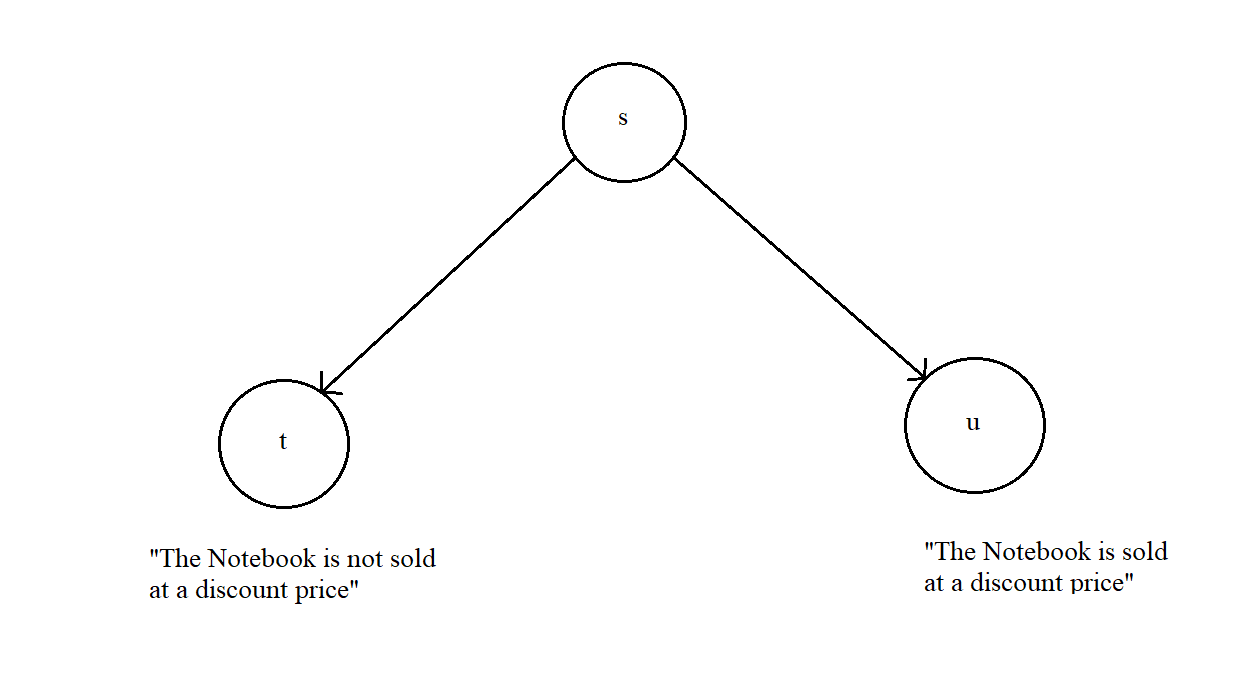
\includegraphics[scale=0.25]{incomplete-modal.png}
%         \caption{A Propositional Modal Logic Model}
%         \label{fig:Modal_Example}
%     \end{figure}\pause
%     Here, at vertex $s$, the seller does not \textbf{know} that "The Notebook is sold at a discount price"
%     % $M,w_3\vDash\Box q$\par\pause
%     % $M,w_1\vDash\Diamond q$\par\pause
%     % $M,w_1\vDash\Diamond\Box q$
% \end{frame}

% \begin{frame}{Introduction: Propositional Modal Logic}
%     \begin{figure}
%         \centering
%         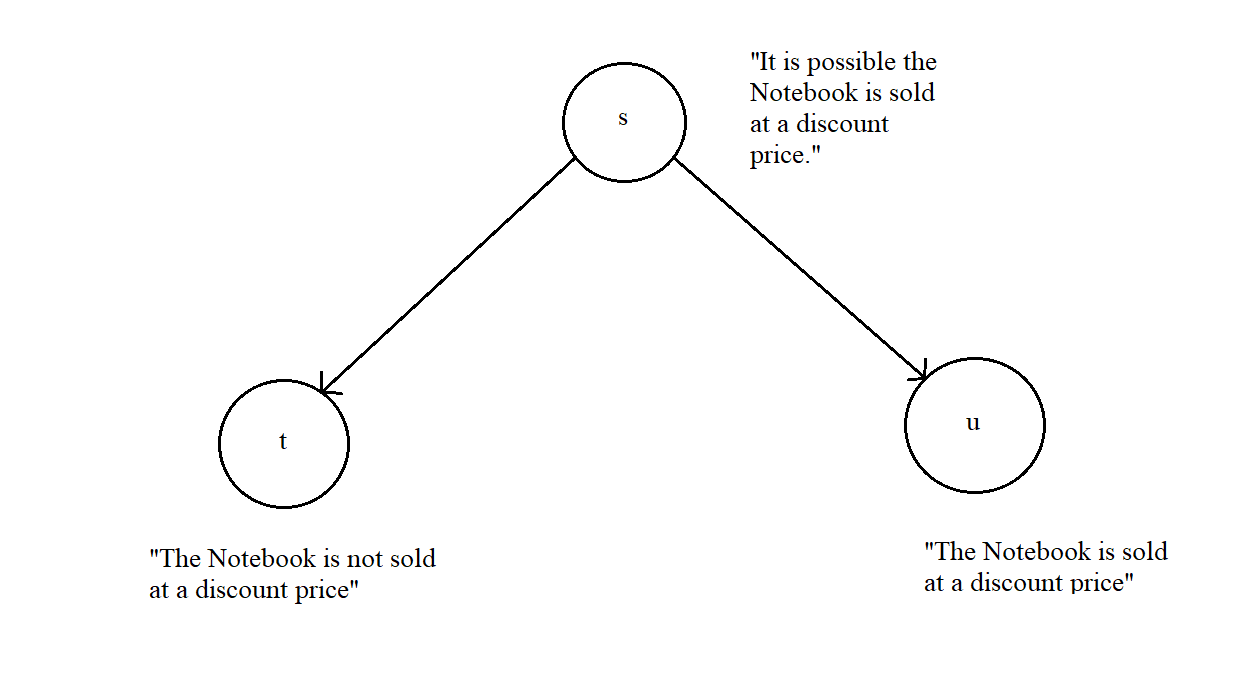
\includegraphics[scale=0.25]{incomplete-modal-pos.png}
%         \caption{A Propositional Modal Logic Model}
%         \label{fig:Modal_Example}
%     \end{figure}
%     Here, at vertex $s$, the seller does not \textbf{know} that "The Notebook is sold at a discount price"\par
%     But believes it is \textbf{possible} that it is sold at a discount price.
%     % $M,w_3\vDash\Box q$\par\pause
%     % $M,w_1\vDash\Diamond q$\par\pause
%     % $M,w_1\vDash\Diamond\Box q$
% \end{frame}

% \begin{frame}{Introduction: Propositional Modal Logic}
%     \begin{figure}
%         \centering
%         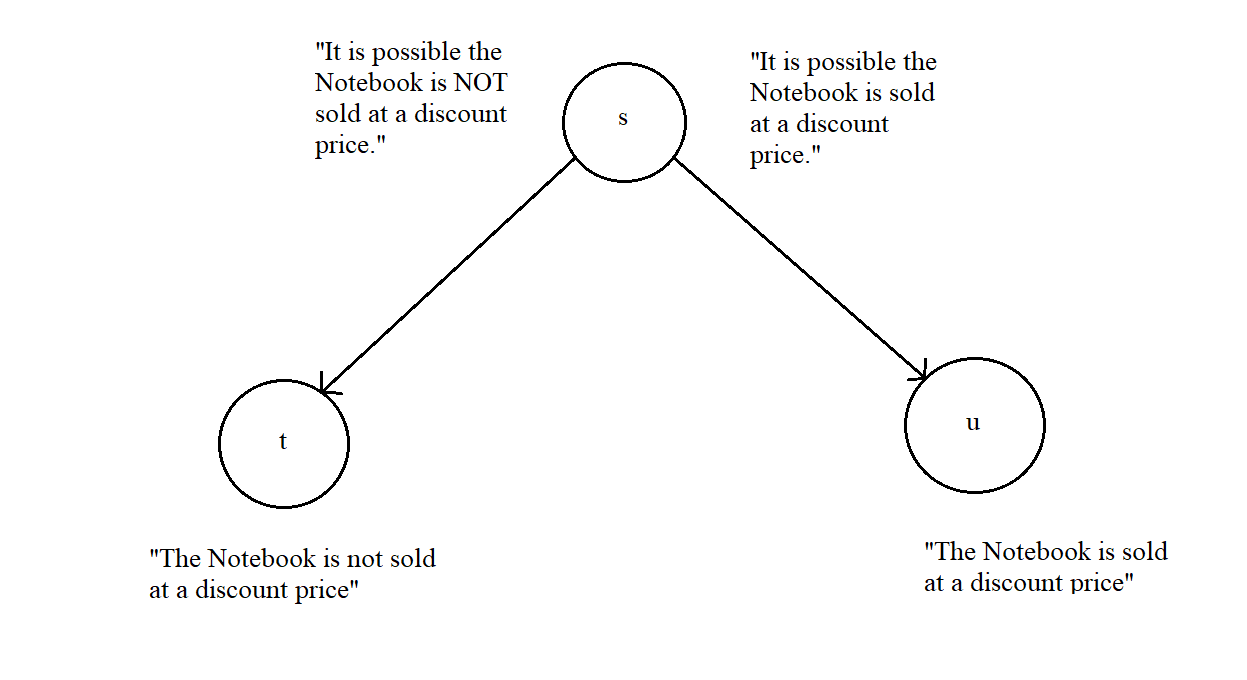
\includegraphics[scale=0.25]{complete-modal.png}
%         \caption{A Propositional Modal Logic Model}
%         \label{fig:Modal_Example}
%     \end{figure}
%     Here, at vertex $s$, the seller does not \textbf{know} that "The Notebook is sold at a discount price"\par
%     But believes it is \textbf{possible} that it is sold at a discount price.\par
%     It is also possible that it is NOT.
%     % $M,w_3\vDash\Box q$\par\pause
%     % $M,w_1\vDash\Diamond q$\par\pause
%     % $M,w_1\vDash\Diamond\Box q$
% \end{frame}


% \begin{frame}{Few Variants of Modal Logic}
%     \begin{itemize}
%         \item<1-> Epistemic Logic: Suppose $A$ is given a card it can see from a pair $\{C_1, C_2 \}$ and other is put on table. Here $A$ \textbf{knows} which card is on the table.
%         \item<2-> Multi-Agent Epistemic Logic: Suppose $A, B$ and $C$ are dealt cards from $\{C_1, C_2, C_3\}$ and cannot see any card other than the one dealt to self. Say $A$ got $C_1$, hence it is an \textbf{epistemic possibility} for $A$ that $B$ is dealt $C_2$, but it a \textbf{knowledge} that $A$ itself has $C_1$.
%     \end{itemize}
% \end{frame}

% \begin{frame}{Relevant Questions}
%     \begin{itemize}
%         \item<1-> Decidability and Complexity of the Model-Checking Problem: Given a model (pointed, in modal logic) and a formula, does the model satisfy the formula?
%         \item<2-> Decidability and Complexity of the Satisfiability Problem: Given a formula, does there exist a model that satisfies it?
%         \item<3-> Expressibility of the system: What properties can the system express?
%         \item<4-> Succinctness of the system: Compared to formulas in other systems, how much larger or smaller sized but equivalent formulas can the system represent?  
%     \end{itemize}
% \end{frame}

% \begin{frame}{Introduction: A Scenario}
%   \textbf{Fun Fact:} In France, the traffic light sequence is a bit different than other parts of Europe. It goes like (green$^*$-amber-red$^*$)$^*$, whereas in most of other parts of Europe it is like (green$^*$-amber-red$^*$-amber)$^*$\par\pause
   
%   Consider a traveller travelling from Switzerland to France. She expects (green$^*$-amber-red$^*$)$^*$ sequence and hence she will know she is in France. Else she is expecting (green$^*$-amber-red$^*$-amber)$^*$ in Switzerland.\\\pause
%   \begin{figure}
%       \centering
%         \begin{tikzpicture}[node distance = 8cm]
%             \node(s) [fastate, minimum size = 2cm, label = 180:$s$]{$f$};
%             \node(t) [fastate, minimum size = 2cm, right of = s, label = 0:$t$]{$\neg{f}$};
            
%             \node(franceExp) [rectNode, yshift = 6.5cm, below of=s]{$(g^*ar^*)^*$};
%             \node(EuroExp) [rectNode, yshift = 6.5cm, below of=t]{$(g^*ar^*a)^*$};
            
%             \draw[-](s.east)--node[anchor=south]{$Traveller$}(t.west);
    
%         \end{tikzpicture}
%       \caption{The Model of the scenario. $f$ stands for France, hence $\neg{f}$ is NOT in France.}
%   \end{figure}
% \end{frame}

% \begin{frame}{Introduction: A Scenario}
%     Suppose the traveller observes that the traffic signal sequence $garg$, that is, the red switches to green without an amber transition in the middle.\par\pause
    
%     What does she deduce?\pause She is in France.\\\pause
    
%     \begin{figure}
%       \centering
%         \begin{tikzpicture}[node distance = 2cm]
%             \node(s) [fastate, minimum size = 2cm, label = 180:$s$]{$f$};
            
%             \node(franceExp) [rectNode, yshift = .5cm, below of=s]{$(g^*ar^*)^*$};
            
%             \draw[->](s.north)..controls +(up:2cm) and +(right:2cm)..node[anchor=west]{$Traveller$}(s.east);
    
%         \end{tikzpicture}
%       \caption{The Model of the updated scenario. $f$ stands for France, hence $\neg{f}$ is NOT in model.}
%   \end{figure}
% \end{frame}

% \begin{frame}{A Formal Model}
%     A POL model $\M = \ldiaarg{W, R, V, Exp}$ is a relational structure:
%     \begin{itemize}
%         \item<1-> A set of worlds $W$.
%         \item<2-> A set of relations $R$. 
%         \begin{itemize}
%             \item<3-> For every $\sim_i\in R$, $\sim_i\subseteq W\times W$ and is an equivalence relation, over all agents $i\in Agt$.
%         \end{itemize}
        
%         \item<4-> An assignment of propositional letters $\mathcal{P}$ for each world ($V:W\rightarrow 2^{\mathcal{P}}$).
        
%         \item<5-> A regular expression in each world representing the expectations in the world. ($Exp$). 
        
%         \item<6-> Can be visualized as graph:
%         \begin{itemize}
%             \item<7-> Each node (world) labelled with assignments and expectation.
%             \item<8-> Edges are relation labelled by agent.
%         \end{itemize}
%     \end{itemize}
    
% \end{frame}

% \begin{frame}{An Observation: How the model updates?}
%     After an observation, the model was updated.\par\pause
%     \textbf{How?}\par\pause
%     Consider a regular expression $\pi$ and a word $w$.\par\pause
%     Residue $\pi\setminus w$: Regular expression for all the words $u$ such that:\\\pause
%     $wu$ was a word in $\pi$.\par\pause
%     For example, $\pi = abb + baa$ and $w = ab$\\
%     $\pi\setminus w = b$.
% \end{frame}

% \begin{frame}{Model Updation}
%     Given a word $w$ and model $\M$, in the model $\M|_w$\par\pause
%     A world $s$ survives iff $\LL(Exp(s)\setminus w)$ is not an empty language.\par\pause
%     A world disappears along all its relations.\par\pause
%     Each surviving world $s$ has its new expectation as $Exp(s)\setminus w$
% \end{frame}

% \begin{frame}{Model Updation}
%     Consider the model in our previous example:\\\pause
%     \begin{tikzpicture}[node distance = 8cm]
%             \node(s) [fastate, minimum size = 2cm, label = 180:$s$]{$f$};
%             \node(t) [fastate, minimum size = 2cm, right of = s, label = 0:$t$]{$\neg{f}$};
            
%             \node(franceExp) [rectNode, yshift = 6.5cm, below of=s]{$(g^*ar^*)^*$};
%             \node(EuroExp) [rectNode, yshift = 6.5cm, below of=t]{$(g^*ar^*a)^*$};
            
%             \draw[-](s.east)--node[anchor=south]{$Traveller$}(t.west);
    
%     \end{tikzpicture}\\\pause
%     Then the observation arrives $garg$\par\pause
    
%     Note that, $(g^*ar^*a)^*\setminus garg = \delta$\\\pause
%     \begin{tikzpicture}
%             \node(s) [fastate, minimum size = 1cm, label = 180:$s$, yshift = 2cm]{$f$};
            
%             \node(franceExp) [rectNode, right of=s, xshift =1cm]{$(g^*ar^*)^*$};
            
%             \draw[->](s.north)..controls +(up:2cm) and +(right:2cm)..node[anchor=west]{$Traveller$}(s.east);
    
%         \end{tikzpicture}
% \end{frame}

% \begin{frame}{Introduction: POL Syntax}
%     How do formulas in POL look?\par\pause
    
%     Will contain formulas that look like proposition logic\\\pause
%     $\varphi\vee\psi$,$\varphi\wedge\psi$,$\neg{\varphi}$ over some propositional letters $\mathcal{P}$.\pause\par
    
%     Also a linear operator $\hat{K_i}$ for every agent $i$.\\\pause
%     This operator is required for interpreting knowledge of agents.\\
%     $\hat{K_i}\varphi$.\par\pause
    
%     Another linear operator $\ldiaarg{\pi}$ for a regular expression $\pi$.\\\pause
%     This operator to denote an observation as occurred, after that whether $\varphi$ is a truth .\\
%     $\ldiaarg{\pi}\varphi$.
% \end{frame}

% \begin{frame}{Introduction: Semantics}
%     What do these formula mean? \par\pause

%     \textbf{Meaning} brings \textbf{Interpretation}\\\pause
%     And \textbf{Interpretation} brings \textbf{Model}.\par\pause
    
%     Whether the interpretation stated by the formula it true is evaluated in this model.
% \end{frame}

% \begin{frame}{Semantics}
% A formula $\varphi$ is true in world $s$ of $\M$ iff
%     \begin{itemize}
%         \item<1-> $\varphi = p\in\mathcal{P}$, $p$ is assigned $True$ in $s$ ($p\in V(s)$).
        
%         \item<2-> $\varphi = \psi_1\vee\psi_2$, $\psi_1$ is $True$ in $s$ OR $\psi_2$ is $True$ in $s$.
        
%         \item<3-> $\varphi = \neg{\psi}$, $\psi$ is NOT $True$ in $s$.
        
%         \item<4-> $\varphi = \hat{K_i}\psi$, there EXISTS a world $t$ related to $s$ where $\psi$ is $True$.
        
%         \item<5-> $\varphi = \ldiaarg{\pi}\psi$, there EXISTS an observation $w$ in $\pi$ such that $s$ survives in $\M|_w$ and $\psi$ is $True$ in the residue.
%     \end{itemize}
% \end{frame}

% \begin{frame}{Semantics}
%     There are some universal linear operators used corresponding to the existential linear operators.\par\pause
    
%     $K_i\varphi = \neg{\hat{K_i}\neg{\varphi}}$\\\pause
%     Hence $K_i\varphi$ is $True$ in world $s$ of $\M$ iff\\\pause
%     For all related worlds $t$ with $s$, $\varphi$ is $True$ in them.\par\pause
    
%     $[\pi]\varphi = \neg{\ldiaarg{\pi}\neg{\varphi}}$\\\pause
%     Hence $[\pi]\varphi$ is $True$ in world $s$ of $\M$ iff\\\pause
%     For all word $w$ in $\pi$, if $s$ survives in $\M|_w$ then $\varphi$ is $True$ in it.
% \end{frame}

% \begin{frame}{Example formulas}
%     Consider a few example formulas from our example that is $True$ in our model setting:\par\pause
    
%     $[g^*]\neg(K_T f \lor K_T \neg f)$\pause says that after repetitions of $g$ is observed, $Traveller$ is still uncertain whether she is in France or Switzerland.\par\pause
    
%     $\ldiaarg{(garg)^*}(K_T f)$\pause says there exists an observation in $(garg)^*$ that can make traveller certain that she is in France.
% \end{frame}
\begin{frame}{Background on Public Observation Logic}
    Public Observation Logic (POL) is a logical framework involving
    \begin{itemize}
        \item Multiple Agents
        \item Public Observation
        \item Agents have expectations about observation
        \item Reasoning about knowledge ($K_i\varphi$) after observation.
        \item Possible world (Kripke) semantics
        \item Truncation of possible worlds based on expectation and the public observation
    \end{itemize}
\end{frame}

\begin{frame}{Background on Public Observation Logic}
    \begin{figure}
        \centering
        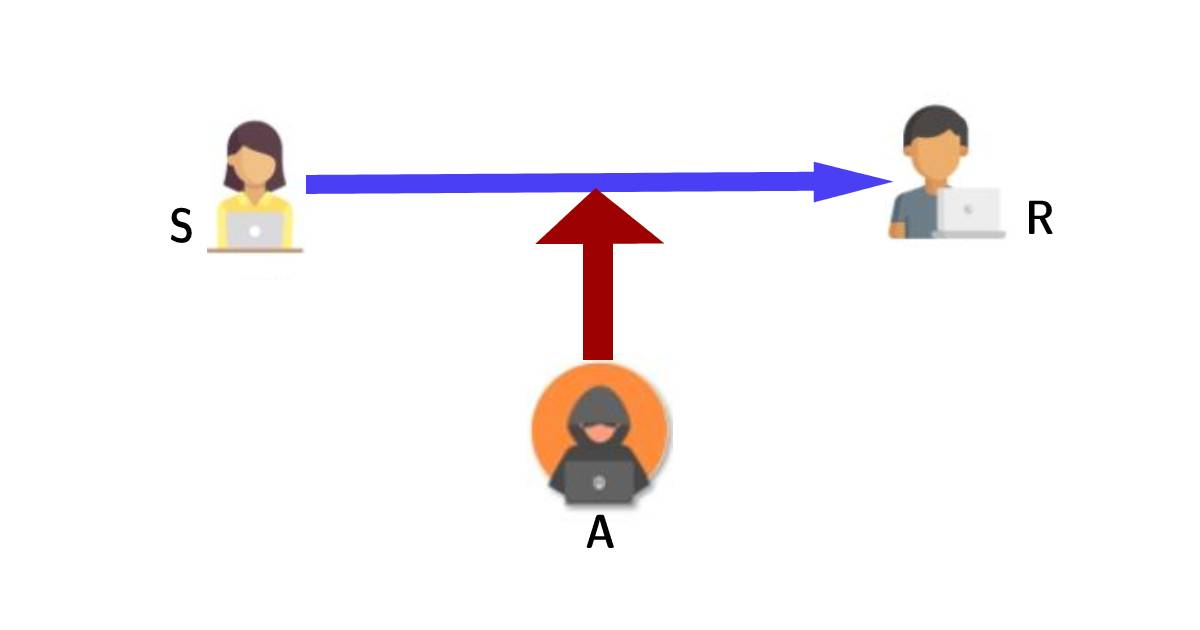
\includegraphics[scale=0.15]{images/comm-slide.jpg}
        \label{fig:my_label}
    \end{figure}
\end{frame}

\begin{frame}{Background on Public Observation Logic}
    \begin{figure}
        \centering
        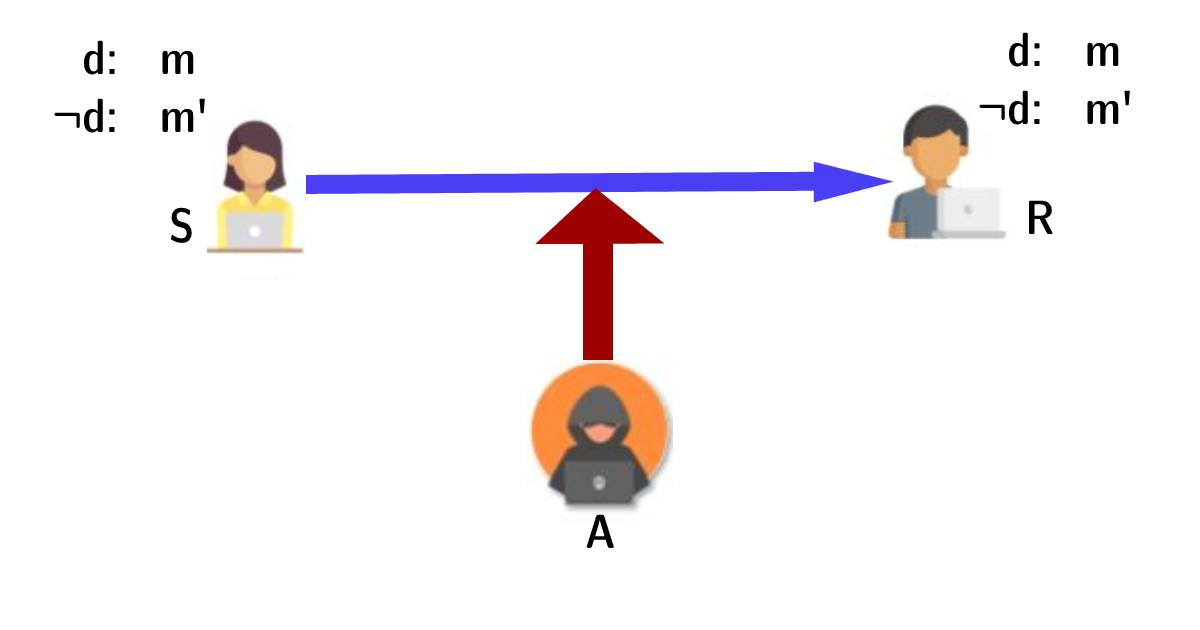
\includegraphics[scale=0.15]{images/comm-slide-srexpect.jpg}
        \label{fig:my_label}
    \end{figure}
\end{frame}

\begin{frame}{Background on Public Observation Logic}
    \begin{figure}
        \centering
        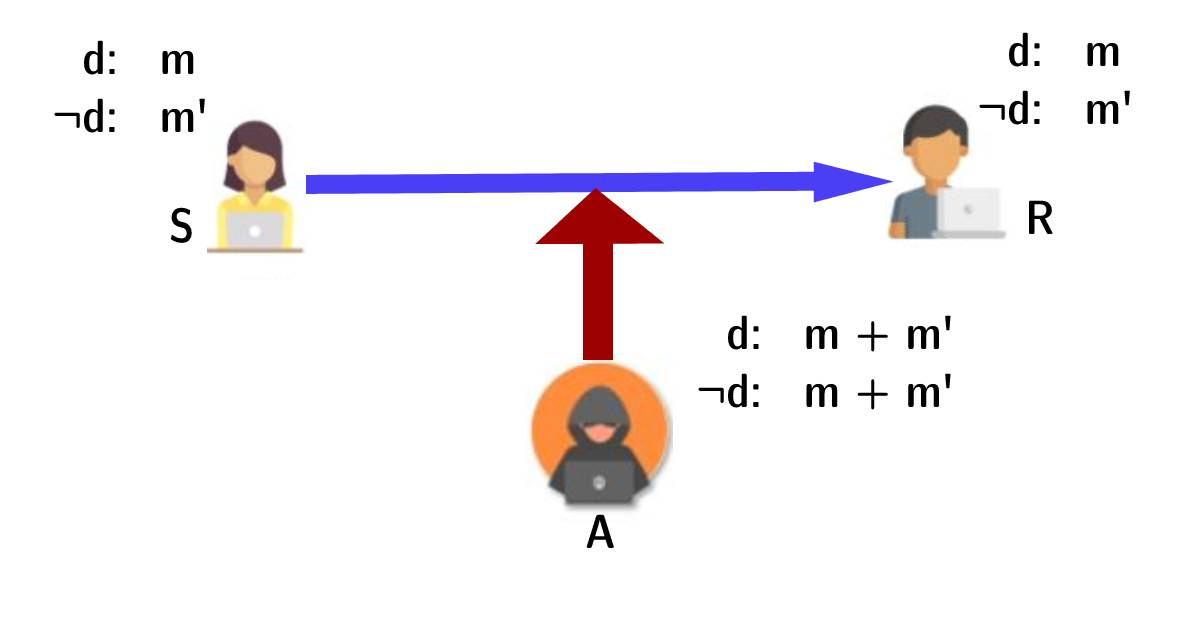
\includegraphics[scale=0.15]{images/comm-slide-allexpect.jpg}
        \label{fig:my_label}
    \end{figure}
\end{frame}

\begin{frame}{Background on Public Observation Logic}
    \begin{figure}
        \begin{center}
            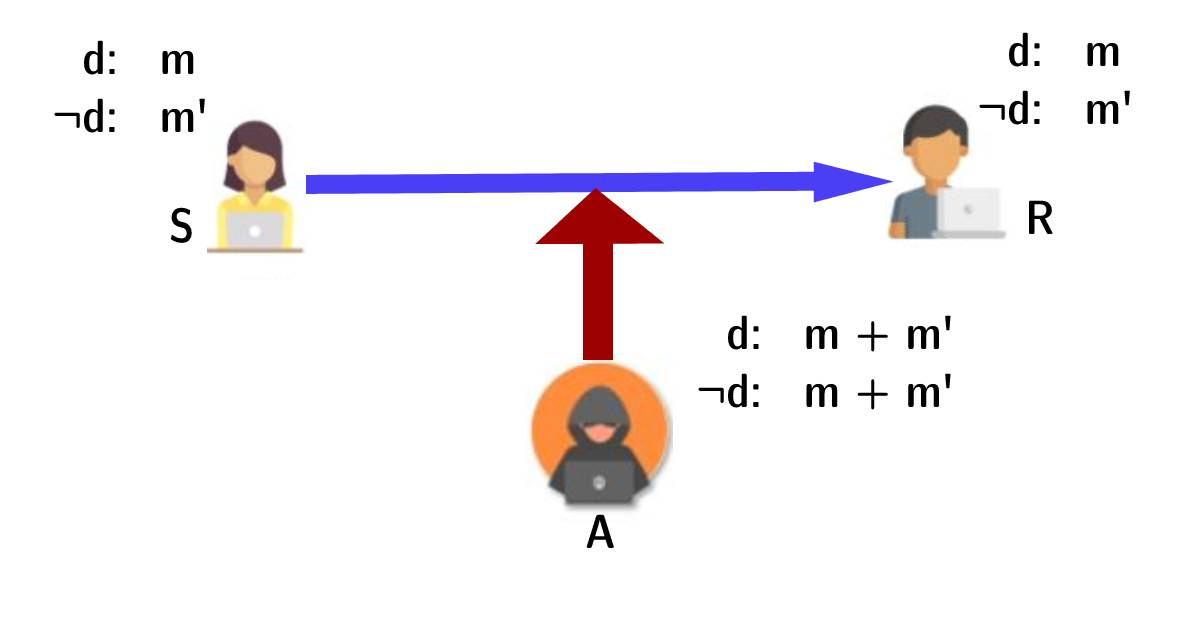
\includegraphics[scale=0.13]{images/comm-slide-allexpect.jpg}
            \begin{tikzpicture}[yscale=1.4]
    				\node[world] (s) {$d$};
    				\node[world] (t) at (4, 0) {$\lnot d$};
    				\node[world] (u) at (0, -1) {$d$};
    				\node[world] (v) at (4, -1) {$\lnot d$};
    				\node[left = 0mm of s] {\underline{$s$}};
    				\node[right = 0mm of t] {$t$};
    				\node[left = 0mm of u] {$u$};
    				\node[right = 0mm of v] {$v$};
    				\node[above = 0mm of s] {$m$};
    				\node[above = 0mm of t] {$m'$};
    				\node[below = 0mm of u] {$m+m'$};
    				\node[below = 0mm of v] {$m+m'$};
    				\draw (s) edge node[above] {$R, A$} (t);
    				\draw (u) edge node[above] {$R, A$} (v);
    				\draw (s) edge node[left] {$A$} (u);
    				\draw (t) edge node[right] {$A$} (v);
    		\end{tikzpicture}
		\end{center}
    \end{figure}\pause
    \begin{figure}
        \begin{center}
            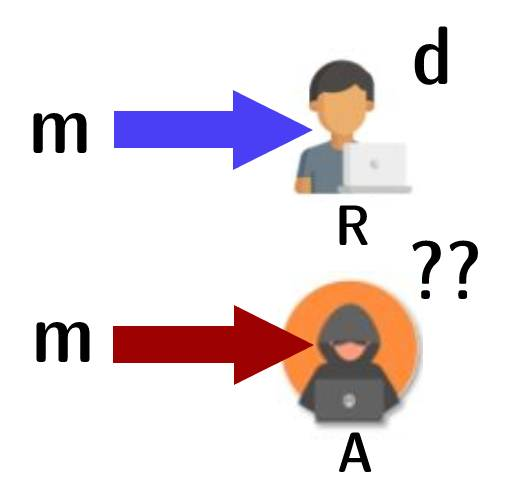
\includegraphics[scale=0.13]{images/rec-observe.jpg}
            \hspace*{40pt}
            \begin{tikzpicture}[yscale=1.4]
    				\node[world] (s) {$d$};
    				\node[world] (u) at (0, -1) {$d$};
    				\node[world] (v) at (4, -1) {$\lnot d$};
    				\node[left = 0mm of s] {\underline{$s$}};
    				\node[left = 0mm of u] {$u$};
    				\node[right = 0mm of v] {$v$};
    				\node[above = 0mm of s] {$\ep$};
    				\node[below = 0mm of u] {$\ep$};
    				\node[below = 0mm of v] {$\ep$};
    				\draw (u) edge node[above] {$R, A$} (v);
    				\draw (s) edge node[left] {$A$} (u);
    		\end{tikzpicture}
		\end{center}
    \end{figure}\pause
    $$\mathcal{M},s\vDash[m](K_R d\wedge \neg{K_A d})$$
\end{frame}

\begin{frame}{Our Contribution}
    Our contribution in this work:
    \begin{itemize}
        \item Complexity result for model checking for $\POL$.
        \item Investigate various syntactic fragments of $\POL$ and their model-checking complexity.
        \item An implementation of model checking of an easier fragment via reduction to SAT.
    \end{itemize}
\end{frame}

\begin{frame}{Purpose of our study: A Farming Drone}
    Consider a farming drone in the maze
    \begin{figure}
	\begin{center}
		\newcommand{\sizefield}{7}
		\begin{tikzpicture}[scale=0.5]
			\foreach \x in {0, 1, ..., \sizefield} {
				\draw (\x, 0) -- (\x, \sizefield);
				\draw (0, \x) -- (\sizefield, \x);
			}
			\node at (0.5, 0.5) {
\includegraphics[width=0.3cm]{images/E097_color.png}};%power
			\node at (6.5, 6.5) {
\includegraphics[width=0.3cm]{images/1F4A7_color.png}};%water
			\node at (3.5, 3.5) {
\includegraphics[width=0.3cm]{images/E1D2_color.png}};%drone
		\end{tikzpicture}
	\end{center}
    \end{figure}
\end{frame}

\begin{frame}{Purpose of our study: A Farming Drone}
    Consider a farming drone in the maze
    \begin{figure}
	\begin{center}
		\newcommand{\sizefield}{7}
		\begin{tikzpicture}[scale=0.5]
			\foreach \x in {0, 1, ..., \sizefield} {
				\draw (\x, 0) -- (\x, \sizefield);
				\draw (0, \x) -- (\sizefield, \x);
			}
			\node at (0.5, 0.5) {
\includegraphics[width=0.3cm]{images/E097_color.png}};%power
			\node at (6.5, 6.5) {
\includegraphics[width=0.3cm]{images/1F4A7_color.png}};%water
			\node at (3.5, 3.5) {
\includegraphics[width=0.3cm]{images/E1D2_color.png}};%drone
		\end{tikzpicture}
		\begin{tikzpicture}[scale=0.5]
			\foreach \x in {0, 1, ..., \sizefield} {
				\draw (\x, 0) -- (\x, \sizefield);
				\draw (0, \x) -- (\sizefield, \x);
			}
			\node at (0.5, 0.5) {
\includegraphics[width=0.3cm]{images/E097_color.png}};%power
			\node at (6.5, 6.5) {
\includegraphics[width=0.3cm]{images/1F4A7_color.png}};%water
			\node at (2.5, 3.5) {
\includegraphics[width=0.3cm]{images/E1D2_color.png}};%drone
		\end{tikzpicture}
	\end{center}
    \end{figure}
    The drone can move left ($\obsleft$)
\end{frame}
\begin{frame}{Purpose of our study: A Farming Drone}
    Consider a farming drone in the maze
    \begin{figure}
	\begin{center}
		\newcommand{\sizefield}{7}
		\begin{tikzpicture}[scale=0.5]
			\foreach \x in {0, 1, ..., \sizefield} {
				\draw (\x, 0) -- (\x, \sizefield);
				\draw (0, \x) -- (\sizefield, \x);
			}
			\node at (0.5, 0.5) {
\includegraphics[width=0.3cm]{images/E097_color.png}};%power
			\node at (6.5, 6.5) {
\includegraphics[width=0.3cm]{images/1F4A7_color.png}};%water
			\node at (3.5, 3.5) {
\includegraphics[width=0.3cm]{images/E1D2_color.png}};%drone
		\end{tikzpicture}
		\begin{tikzpicture}[scale=0.5]
			\foreach \x in {0, 1, ..., \sizefield} {
				\draw (\x, 0) -- (\x, \sizefield);
				\draw (0, \x) -- (\sizefield, \x);
			}
			\node at (0.5, 0.5) {
\includegraphics[width=0.3cm]{images/E097_color.png}};%power
			\node at (6.5, 6.5) {
\includegraphics[width=0.3cm]{images/1F4A7_color.png}};%water
			\node at (4.5, 3.5) {
\includegraphics[width=0.3cm]{images/E1D2_color.png}};%drone
		\end{tikzpicture}
	\end{center}
    \end{figure}
    The drone can move left ($\obsleft$)\\
    The drone can move right ($\obsright$)
\end{frame}

\begin{frame}{Purpose of our study: A Farming Drone}
    Consider a farming drone in the maze
    \begin{figure}
	\begin{center}
		\newcommand{\sizefield}{7}
		\begin{tikzpicture}[scale=0.5]
			\foreach \x in {0, 1, ..., \sizefield} {
				\draw (\x, 0) -- (\x, \sizefield);
				\draw (0, \x) -- (\sizefield, \x);
			}
			\node at (0.5, 0.5) {
\includegraphics[width=0.3cm]{images/E097_color.png}};%power
			\node at (6.5, 6.5) {
\includegraphics[width=0.3cm]{images/1F4A7_color.png}};%water
			\node at (3.5, 3.5) {
\includegraphics[width=0.3cm]{images/E1D2_color.png}};%drone
		\end{tikzpicture}
		\begin{tikzpicture}[scale=0.5]
			\foreach \x in {0, 1, ..., \sizefield} {
				\draw (\x, 0) -- (\x, \sizefield);
				\draw (0, \x) -- (\sizefield, \x);
			}
			\node at (0.5, 0.5) {
\includegraphics[width=0.3cm]{images/E097_color.png}};%power
			\node at (6.5, 6.5) {
\includegraphics[width=0.3cm]{images/1F4A7_color.png}};%water
			\node at (3.5, 4.5) {
\includegraphics[width=0.3cm]{images/E1D2_color.png}};%drone
		\end{tikzpicture}
	\end{center}
    \end{figure}
    The drone can move left ($\obsleft$)\\
    The drone can move right ($\obsright$)\\
    The drone can move up ($\obsup$)
\end{frame}

\begin{frame}{Purpose of our study: A Farming Drone}
    Consider a farming drone in the maze
    \begin{figure}
	\begin{center}
		\newcommand{\sizefield}{7}
		\begin{tikzpicture}[scale=0.5]
			\foreach \x in {0, 1, ..., \sizefield} {
				\draw (\x, 0) -- (\x, \sizefield);
				\draw (0, \x) -- (\sizefield, \x);
			}
			\node at (0.5, 0.5) {
\includegraphics[width=0.3cm]{images/E097_color.png}};%power
			\node at (6.5, 6.5) {
\includegraphics[width=0.3cm]{images/1F4A7_color.png}};%water
			\node at (3.5, 3.5) {
\includegraphics[width=0.3cm]{images/E1D2_color.png}};%drone
		\end{tikzpicture}
		\begin{tikzpicture}[scale=0.5]
			\foreach \x in {0, 1, ..., \sizefield} {
				\draw (\x, 0) -- (\x, \sizefield);
				\draw (0, \x) -- (\sizefield, \x);
			}
			\node at (0.5, 0.5) {
\includegraphics[width=0.3cm]{images/E097_color.png}};%power
			\node at (6.5, 6.5) {
\includegraphics[width=0.3cm]{images/1F4A7_color.png}};%water
			\node at (3.5, 2.5) {
\includegraphics[width=0.3cm]{images/E1D2_color.png}};%drone
		\end{tikzpicture}
	\end{center}
    \end{figure}
    The drone can move left ($\obsleft$)\\
    The drone can move right ($\obsright$)\\
    The drone can move up ($\obsup$)\\
    The drone can move down ($\obsdown$)
\end{frame}

\begin{frame}{Purpose of our study: A Farming Drone}
    For agent $A$:
    \begin{figure}
        \centering
        
\includegraphics[scale=0.2]{images/A-expectwater.jpg}
    \end{figure}
    \begin{itemize}
        \item Drone can go up-right fetching water with at most one error step: $\expwater$
    \end{itemize}
\end{frame}

\begin{frame}{Purpose of our study: A Farming Drone}
    For agent $A$:
    \begin{figure}
        \centering
        
\includegraphics[scale=0.2]{images/A-expectwaterpower.jpg}
    \end{figure}
    \begin{itemize}
        \item Drone can go down-left fetching power with at most one error step: $\exppower$
    \end{itemize}
\end{frame}

\begin{frame}{Purpose of our study: A Farming Drone}
    For agent $A$:
    \begin{figure}
        \centering
        
\includegraphics[scale=0.2]{images/A-expectall.jpg}
    \end{figure}
    \begin{itemize}
        \item Drone can keep patrolling in clockwise square fashion: $\exppatrol$
    \end{itemize}
\end{frame}

\begin{frame}{Purpose of our study: A Farming Drone}
    For $B$:
    \begin{figure}
        \centering
        
\includegraphics[scale=0.2]{images/A-expectall.jpg}
        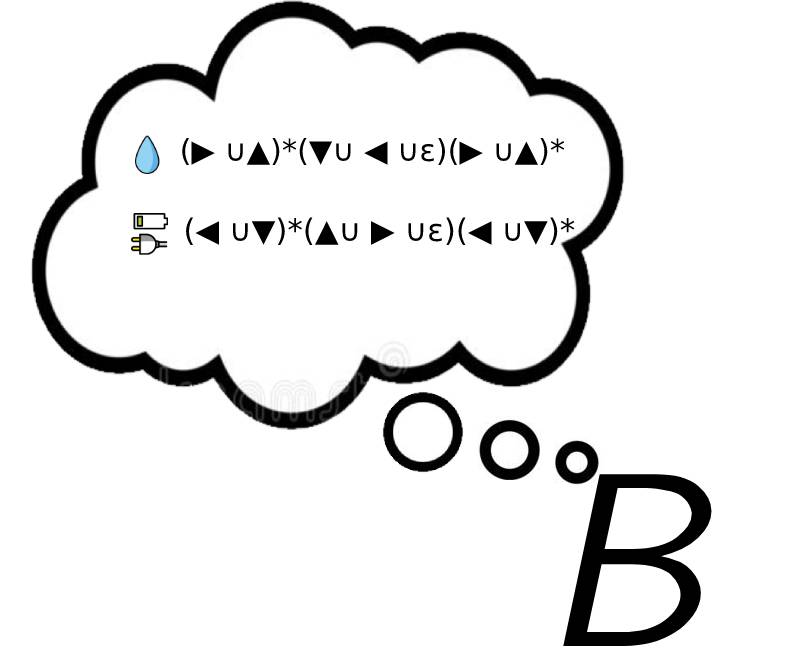
\includegraphics[scale=0.2]{images/B-expectall.jpg}
    \end{figure}
    $B$ expects Drone to go either for power or water.
\end{frame}

\begin{frame}{Purpose of our study: A Farming Drone}
    \begin{figure}
        \centering
        
\includegraphics[scale=0.2]{images/A-expectall.jpg}
        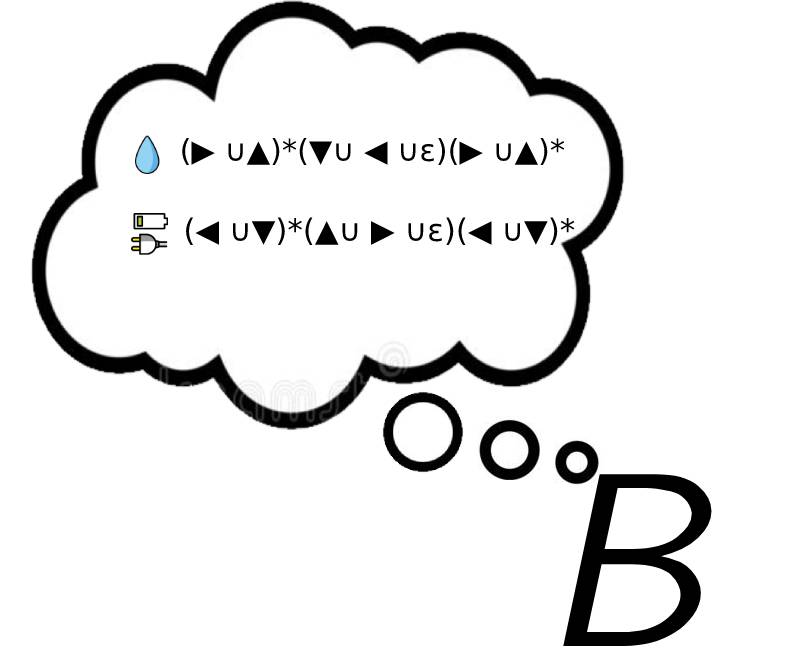
\includegraphics[scale=0.2]{images/B-expectall.jpg}
    \end{figure}
    \begin{figure}
        \begin{tikzpicture}[yscale=1.3]
			\node[world] (s) {$water$};
			\node at (-0.1, -0.4) {\tiny $\expwater$};
			\node[world] (t) at (4, 0) {$power$};
			\node at (4.3, -0.4) {\tiny $\exppower$};
			\node[world] (u) at (0, 1) {$patrol$};
			\node at (2.3, 1) {\tiny $\exppatrol$};
			\node[left = 0mm of s] {\underline{$s$}};
			\node[right = 0mm of t] {$t$};
			\node[left = 0mm of u] {$u$};
			\draw (s) edge node[above] {$a,b$} (t);
			\draw (s) edge node[left] {$a$} (u);
			\draw (t) edge node[above] {$a$} (u);
		\end{tikzpicture}
    \end{figure}
\end{frame}

\begin{frame}{Purpose of our study: A Farming Drone}
    \begin{figure}
		\newcommand{\sizefield}{7}
		\begin{tikzpicture}[scale=0.3]
			\foreach \x in {0, 1, ..., \sizefield} {
				\draw (\x, 0) -- (\x, \sizefield);
				\draw (0, \x) -- (\sizefield, \x);
			}
			\node at (0.5, 0.5) {
\includegraphics[width=0.3cm]{images/E097_color.png}};%power
			\node at (6.5, 6.5) {
\includegraphics[width=0.3cm]{images/1F4A7_color.png}};%water
			\node at (3.5, 3.5) {
\includegraphics[width=0.3cm]{images/E1D2_color.png}};%drone
		\end{tikzpicture}
		\begin{tikzpicture}[yscale=1.3]
			\node[world] (s) {$water$};
			\node at (-0.1, -0.4) {\tiny $\expwater$};
			\node[world] (t) at (4, 0) {$power$};
			\node at (4.3, -0.4) {\tiny $\exppower$};
			\node[world] (u) at (0, 1) {$patrol$};
			\node at (2.3, 1) {\tiny $\exppatrol$};
			\node[left = 0mm of s] {$s$};
			\node[right = 0mm of t] {$t$};
			\node[left = 0mm of u] {$u$};
			\draw (s) edge node[above] {$a,b$} (t);
			\draw (s) edge node[left] {$a$} (u);
			\draw (t) edge node[above] {$a$} (u);
		\end{tikzpicture}
    \end{figure}
    \textbf{Verification of a plan, $\word$ Fragment}:
 	Does the plan $\obsright  \obsright \obsright$ make $A$ aware that drone is fetching water? 
	%
	$$\M, s \models \ldiaarg{\obsright  \obsright \obsright} K_A water$$
\end{frame}

\begin{frame}{Purpose of our study: A Farming Drone}
    \begin{figure}
		\newcommand{\sizefield}{7}
		\begin{tikzpicture}[scale=0.3]
			\foreach \x in {0, 1, ..., \sizefield} {
				\draw (\x, 0) -- (\x, \sizefield);
				\draw (0, \x) -- (\sizefield, \x);
			}
			\node at (0.5, 0.5) {
\includegraphics[width=0.3cm]{images/E097_color.png}};%power
			\node at (6.5, 6.5) {
\includegraphics[width=0.3cm]{images/1F4A7_color.png}};%water
			\node at (3.5, 3.5) {
\includegraphics[width=0.3cm]{images/E1D2_color.png}};%drone
		\end{tikzpicture}
		\begin{tikzpicture}[yscale=1.3]
			\node[world] (s) {$water$};
			\node at (-0.1, -0.4) {\tiny $\expwater$};
			\node[world] (t) at (4, 0) {$power$};
			\node at (4.3, -0.4) {\tiny $\exppower$};
			\node[world] (u) at (0, 1) {$patrol$};
			\node at (2.3, 1) {\tiny $\exppatrol$};
			\node[left = 0mm of s] {$s$};
			\node[right = 0mm of t] {$t$};
			\node[left = 0mm of u] {$u$};
			\draw (s) edge node[above] {$a,b$} (t);
			\draw (s) edge node[left] {$a$} (u);
			\draw (t) edge node[above] {$a$} (u);
		\end{tikzpicture}
    \end{figure}
    \textbf{Epistemic planning, $\existential$ Fragment}:
 Does there exist a plan for the drone such that agent $b$ would know that the drone is searching for water while agent $a$ would still consider patrolling a possibility?
	%
	$$\M, s \models \ldiaarg{(\obsright \union \obsdown \union \obsleft \union \obsup)^*} (K_B water \land \hat K_A patrolling)$$
\end{frame}

\begin{frame}{Purpose of our study: A Farming Drone}
    \begin{figure}
		\newcommand{\sizefield}{7}
		\begin{tikzpicture}[scale=0.3]
			\foreach \x in {0, 1, ..., \sizefield} {
				\draw (\x, 0) -- (\x, \sizefield);
				\draw (0, \x) -- (\sizefield, \x);
			}
			\node at (0.5, 0.5) {
\includegraphics[width=0.3cm]{images/E097_color.png}};%power
			\node at (6.5, 6.5) {
\includegraphics[width=0.3cm]{images/1F4A7_color.png}};%water
			\node at (3.5, 3.5) {\includegraphics[width=0.3cm]{images/E1D2_color.png}};%drone
		\end{tikzpicture}
		\begin{tikzpicture}[yscale=1.3]
			\node[world] (s) {$water$};
			\node at (-0.1, -0.4) {\tiny $\expwater$};
			\node[world] (t) at (4, 0) {$power$};
			\node at (4.3, -0.4) {\tiny $\exppower$};
			\node[world] (u) at (0, 1) {$patrol$};
			\node at (2.3, 1) {\tiny $\exppatrol$};
			\node[left = 0mm of s] {$s$};
			\node[right = 0mm of t] {$t$};
			\node[left = 0mm of u] {$u$};
			\draw (s) edge node[above] {$a,b$} (t);
			\draw (s) edge node[left] {$a$} (u);
			\draw (t) edge node[above] {$a$} (u);
		\end{tikzpicture}
    \end{figure}
    \textbf{Bounded Epistemic planning, $\starfree$ $\existential$ Fragment}:
 Does there exist a plan OF AT MOST 4 MOVES for the drone such that agent $b$ would know that the drone is searching for water while agent $a$ would still consider patrolling a possibility?
	%
	$$\M, s \models \ldiaarg{(\obsright \union \obsdown \union \obsleft \union \obsup)^4} (K_B water \land \hat K_A patrolling)$$
\end{frame}

\begin{frame}{Purpose of our study: A Farming Drone}
    \begin{figure}
		\newcommand{\sizefield}{7}
		\begin{tikzpicture}[scale=0.3]
			\foreach \x in {0, 1, ..., \sizefield} {
				\draw (\x, 0) -- (\x, \sizefield);
				\draw (0, \x) -- (\sizefield, \x);
			}
			\node at (0.5, 0.5) {\includegraphics[width=0.3cm]{images/E097_color.png}};%power
			\node at (6.5, 6.5) {\includegraphics[width=0.3cm]{images/1F4A7_color.png}};%water
			\node at (3.5, 3.5) {\includegraphics[width=0.3cm]{images/E1D2_color.png}};%drone
		\end{tikzpicture}
		\begin{tikzpicture}[yscale=1.3]
			\node[world] (s) {$water$};
			\node at (-0.1, -0.4) {\tiny $\expwater$};
			\node[world] (t) at (4, 0) {$power$};
			\node at (4.3, -0.4) {\tiny $\exppower$};
			\node[world] (u) at (0, 1) {$patrol$};
			\node at (2.3, 1) {\tiny $\exppatrol$};
			\node[left = 0mm of s] {$s$};
			\node[right = 0mm of t] {$t$};
			\node[left = 0mm of u] {$u$};
			\draw (s) edge node[above] {$a,b$} (t);
			\draw (s) edge node[left] {$a$} (u);
			\draw (t) edge node[above] {$a$} (u);
		\end{tikzpicture}
    \end{figure}
    \textbf{$\starfree$ Fragment}:
 Agent $a$ would not gain the knowledge that the drone will search for water with less than or equal to 2 movements but it is possible with 3 movements:
		\begin{align*}
\M, s \models & [(\obsright \union \obsdown \union \obsleft \union \obsup)^2] \lnot K_A water 
 \land\ldiaarg{(\obsright \union \obsdown \union \obsleft \union \obsup)^3} K_A water
		\end{align*}
\end{frame}

\begin{frame}{Purpose of our study: A Farming Drone}
    \begin{figure}
		\newcommand{\sizefield}{7}
		\begin{tikzpicture}[scale=0.3]
			\foreach \x in {0, 1, ..., \sizefield} {
				\draw (\x, 0) -- (\x, \sizefield);
				\draw (0, \x) -- (\sizefield, \x);
			}
			\node at (0.5, 0.5) {\includegraphics[width=0.3cm]{images/E097_color.png}};%power
			\node at (6.5, 6.5) {\includegraphics[width=0.3cm]{images/1F4A7_color.png}};%water
			\node at (3.5, 3.5) {\includegraphics[width=0.3cm]{images/E1D2_color.png}};%drone
		\end{tikzpicture}
		\begin{tikzpicture}[yscale=1.3]
			\node[world] (s) {$water$};
			\node at (-0.1, -0.4) {\tiny $\expwater$};
			\node[world] (t) at (4, 0) {$power$};
			\node at (4.3, -0.4) {\tiny $\exppower$};
			\node[world] (u) at (0, 1) {$patrol$};
			\node at (2.3, 1) {\tiny $\exppatrol$};
			\node[left = 0mm of s] {$s$};
			\node[right = 0mm of t] {$t$};
			\node[left = 0mm of u] {$u$};
			\draw (s) edge node[above] {$a,b$} (t);
			\draw (s) edge node[left] {$a$} (u);
			\draw (t) edge node[above] {$a$} (u);
		\end{tikzpicture}
    \end{figure}
    \textbf{Full Language}:
 It is impossible for the agent $a$ to know that the drone is searching for water with only down and left movements but there is a plan if all movements are allowed:
		\begin{align*}
		\M, s \models & [(\obsdown \union \obsleft)^*] \lnot K_A water 
		\land \ldiaarg{(\obsright \union \obsdown \union \obsleft \union \obsup)^*} K_A water
	\end{align*}
\end{frame}

\begin{frame}{Concluding: The results}
    Our results in the work:
    \begin{figure}
	\begin{center}
		\newcommand{\ybottom}{-1.2}
		\newcommand{\sep}[1]{\draw (####1, 1.6) -- (####1, \ybottom);}
		\tikzstyle{box} = [inner sep=0.4mm]
		\tikzstyle{inclusion} = [-latex, line width=0.5mm]
		\scalebox{0.9}{
			\begin{tikzpicture}[xscale=2.2, yscale=1]
				\draw (-1.4, \ybottom) rectangle (2.8, 1.6);
				\draw (-1.4, 1) -- (2.8, 1);
				\node[text width=3cm,box] (full) at (2.5, 0) {Full language };
				\node[text width=15mm,box] (starfree) at (1.1, 0.5) {$\starfree$ };
				\node[text width=14mm] (exist) at (1.1, -0.5) {$\existential$ };
				\node[text width=15mm] (starfreeexist) at (0, -0.5) {$\starfree$ $\existential$ };
				\node[text width=8mm] (word) at (-1, 0.5) {$\word$ };
				\node at (1.5, 1.2) {$\PSPACE$-complete};
				\node at (0, 1.2) {$\NP$-complete};
				\node at (-1, 1.24) {in $\PTIME$};
				\sep {0.55}
				\sep {-0.6}
				\draw[inclusion] (starfree) -- (full);
				\draw[inclusion] (exist) -- (full);
				\draw[inclusion] (starfreeexist) edge[out=10, in=200] (starfree);
				\draw[inclusion] (starfreeexist) -- (exist);
				\draw[inclusion] (word) -- (starfree);
		\end{tikzpicture}}
	\end{center}
\end{figure}
\end{frame}
\begin{frame}{Thank You}
    \begin{figure}
        \centering
        \includegraphics{images/question.jpg}
    \end{figure}
\end{frame}

\end{document}
